\newpage
\section{Utilizing graph eigenvectors [25 points]}
The entries of the eigenvector associated with the first ($\lambda_1$) and second ($\lambda_2$) smallest of the Laplacian $L$ are plotted in Figure~\ref{fig:eig}. The behaviour of the $\lambda_1$'s eigenvector $v_1$ is expected to have only 1's as its elements due to the property of the $L$. In our case the entries are not 1 but the normalized vector which is  $\frac{v_1}{\sqrt{n}}$, where $n$ is the length of the eigenvector \cite{noauthor_smallest_nodate}. The Fiedler vector $v_2$ of the second smallest eigen value reflects the structure of the graph. Vertices are strongly connected will have similar eigenvector values, while vertices will show more distinct values, when they are further apart. When looking at plot for $v_2$ in the Subfigure \ref{sfig:eig2} you can see that the vector shows a smooth transition from positive to negative indicating that they are transitioning from one partition to another. Subfigure \ref{sfig:eig1} then shows this grouping using coloring of the vertices.
\begin{figure}[H]
	\centering
	\begin{subfigure}{0.5\textwidth}
		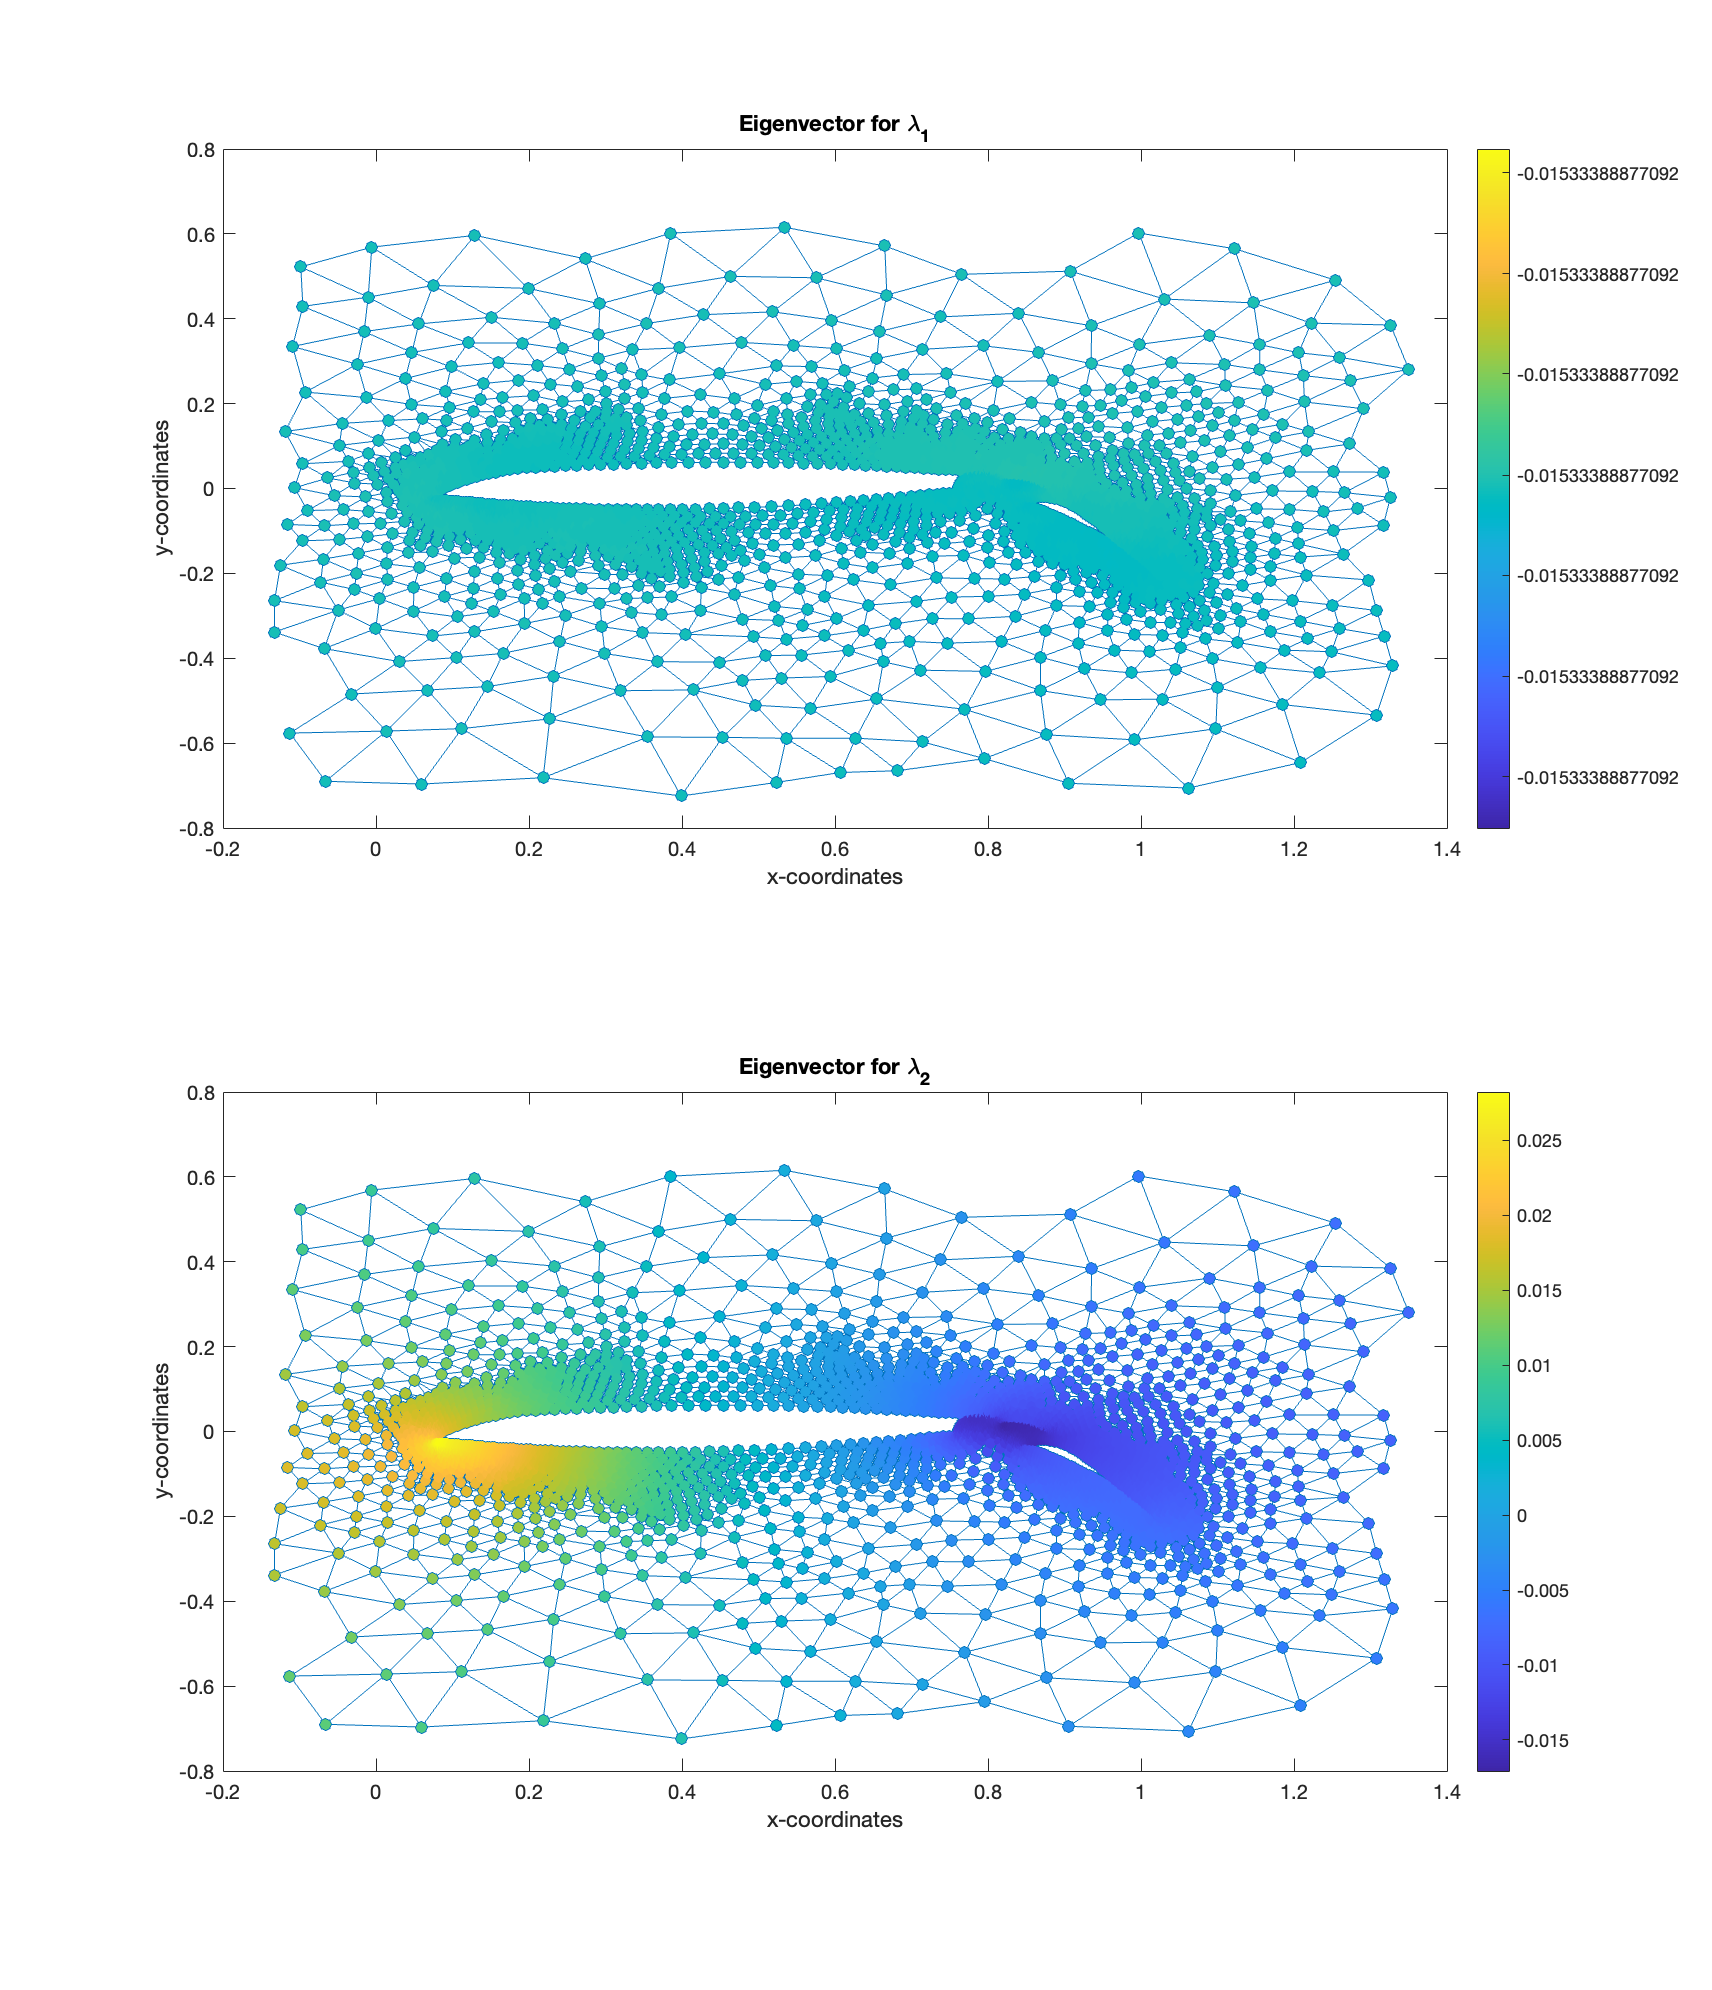
\includegraphics[width=\textwidth]{./media/eigenvector.png}
		\caption{The vertices colored according to their corresponding eigenvector element}
		\label{sfig:eig1}
	\end{subfigure}%
	~
	\begin{subfigure}{0.5\textwidth}
		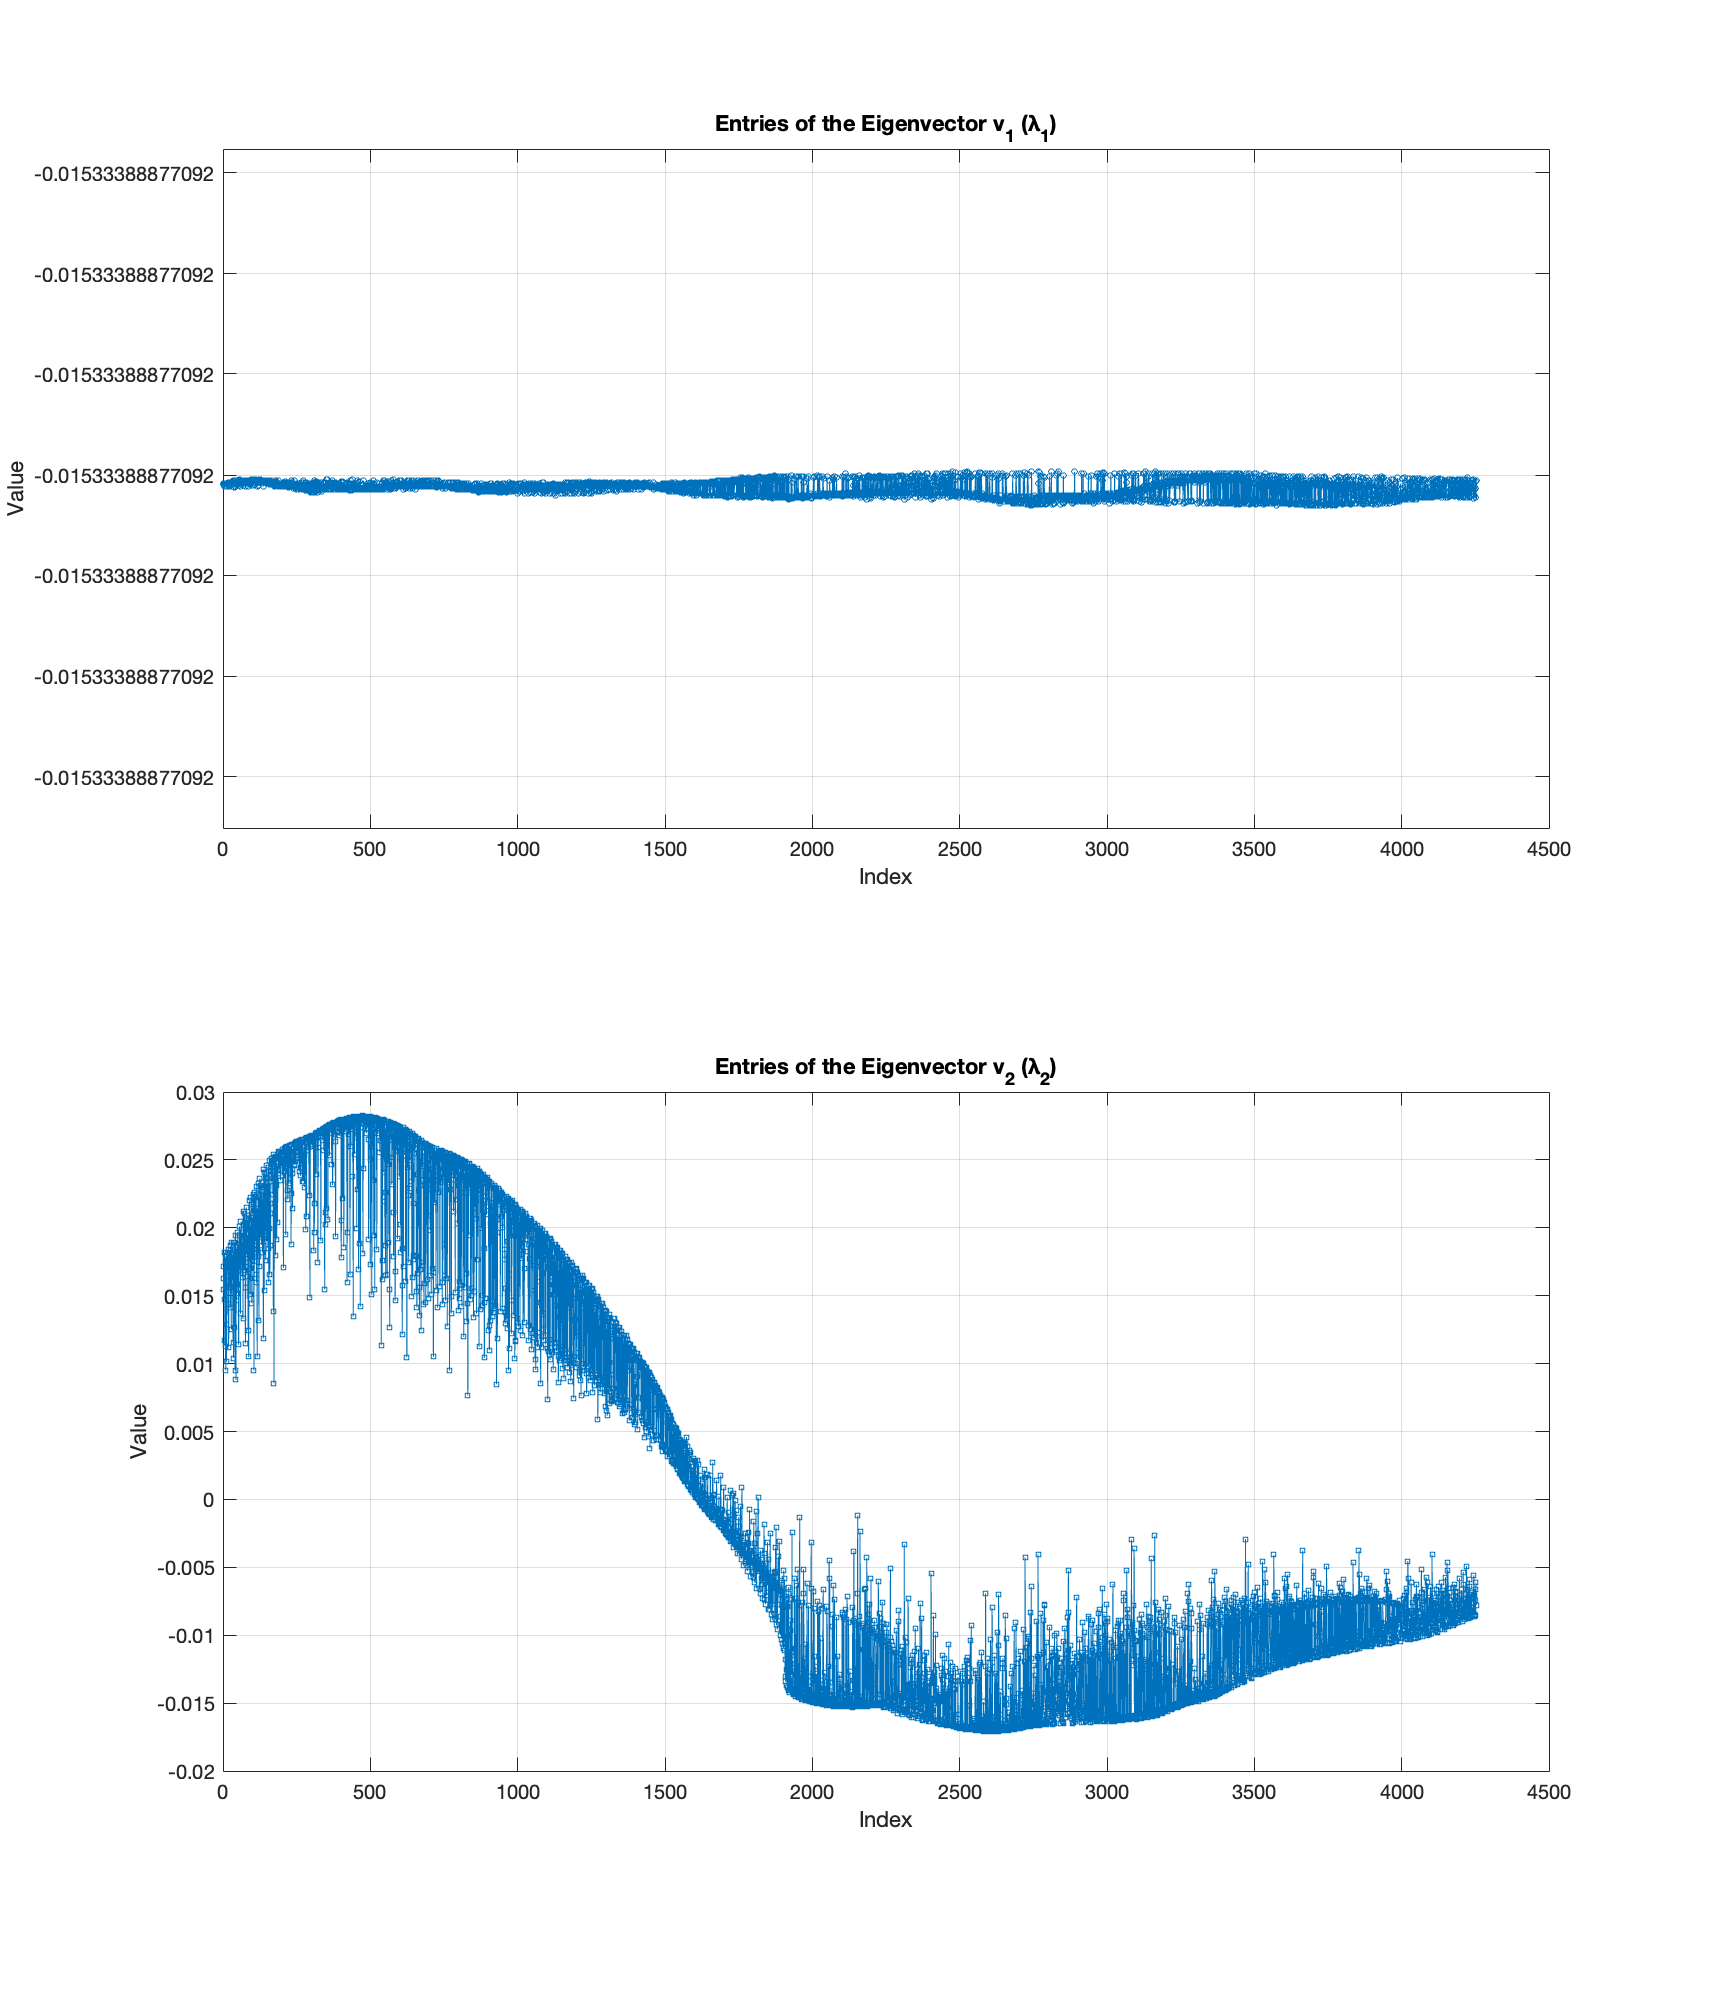
\includegraphics[width=\textwidth]{./media/eig_2.png}
		\caption{The entries of the eigenvector plotted against their indices. }
		\label{sfig:eig2}
	\end{subfigure}\\
	\caption{Entries of the eigenvector associated with the first ($\lambda_1$)} and second ($\lambda_2$) smallest eigenvector.
	\label{fig:eig}
\end{figure}
As the next step we project each solution on the coordinate system space for the graph mesh3e1, barth4, 3elt and crack The result of this can be seen in Figure~\ref{fig:proj}. Looking at the shape of the values of the fiedler vector we can see that the for 3elt and barth4, they are concentrated in a vertical transition.
While for the other two, they have more of a planar structure, creating a clear horizontal separation. Furthermore all graphs appear to have a smooth transition, seen by the transition of color from dark blue to red.
\newline
\newline
As the final step show the graph with its partitions and edge cut by not using the coordinate space, but by using the eigenvectors values of the graph Laplacian.
In Figure~\ref{fig:eig_spc} one can see the partitioning results in two ways. On the top using the eigenvector values and on the bottom the Euclidean coordinates. For the barth4 mesh for example in Subfigure \ref{fig:barth4_spc} we are able to visualize the relation between nodes a lot more effectively using the eigenvector values as our coordinates, in comparison to the cartesian version, where the groups are barely visible. 
\begin{figure}[H]
	\centering
	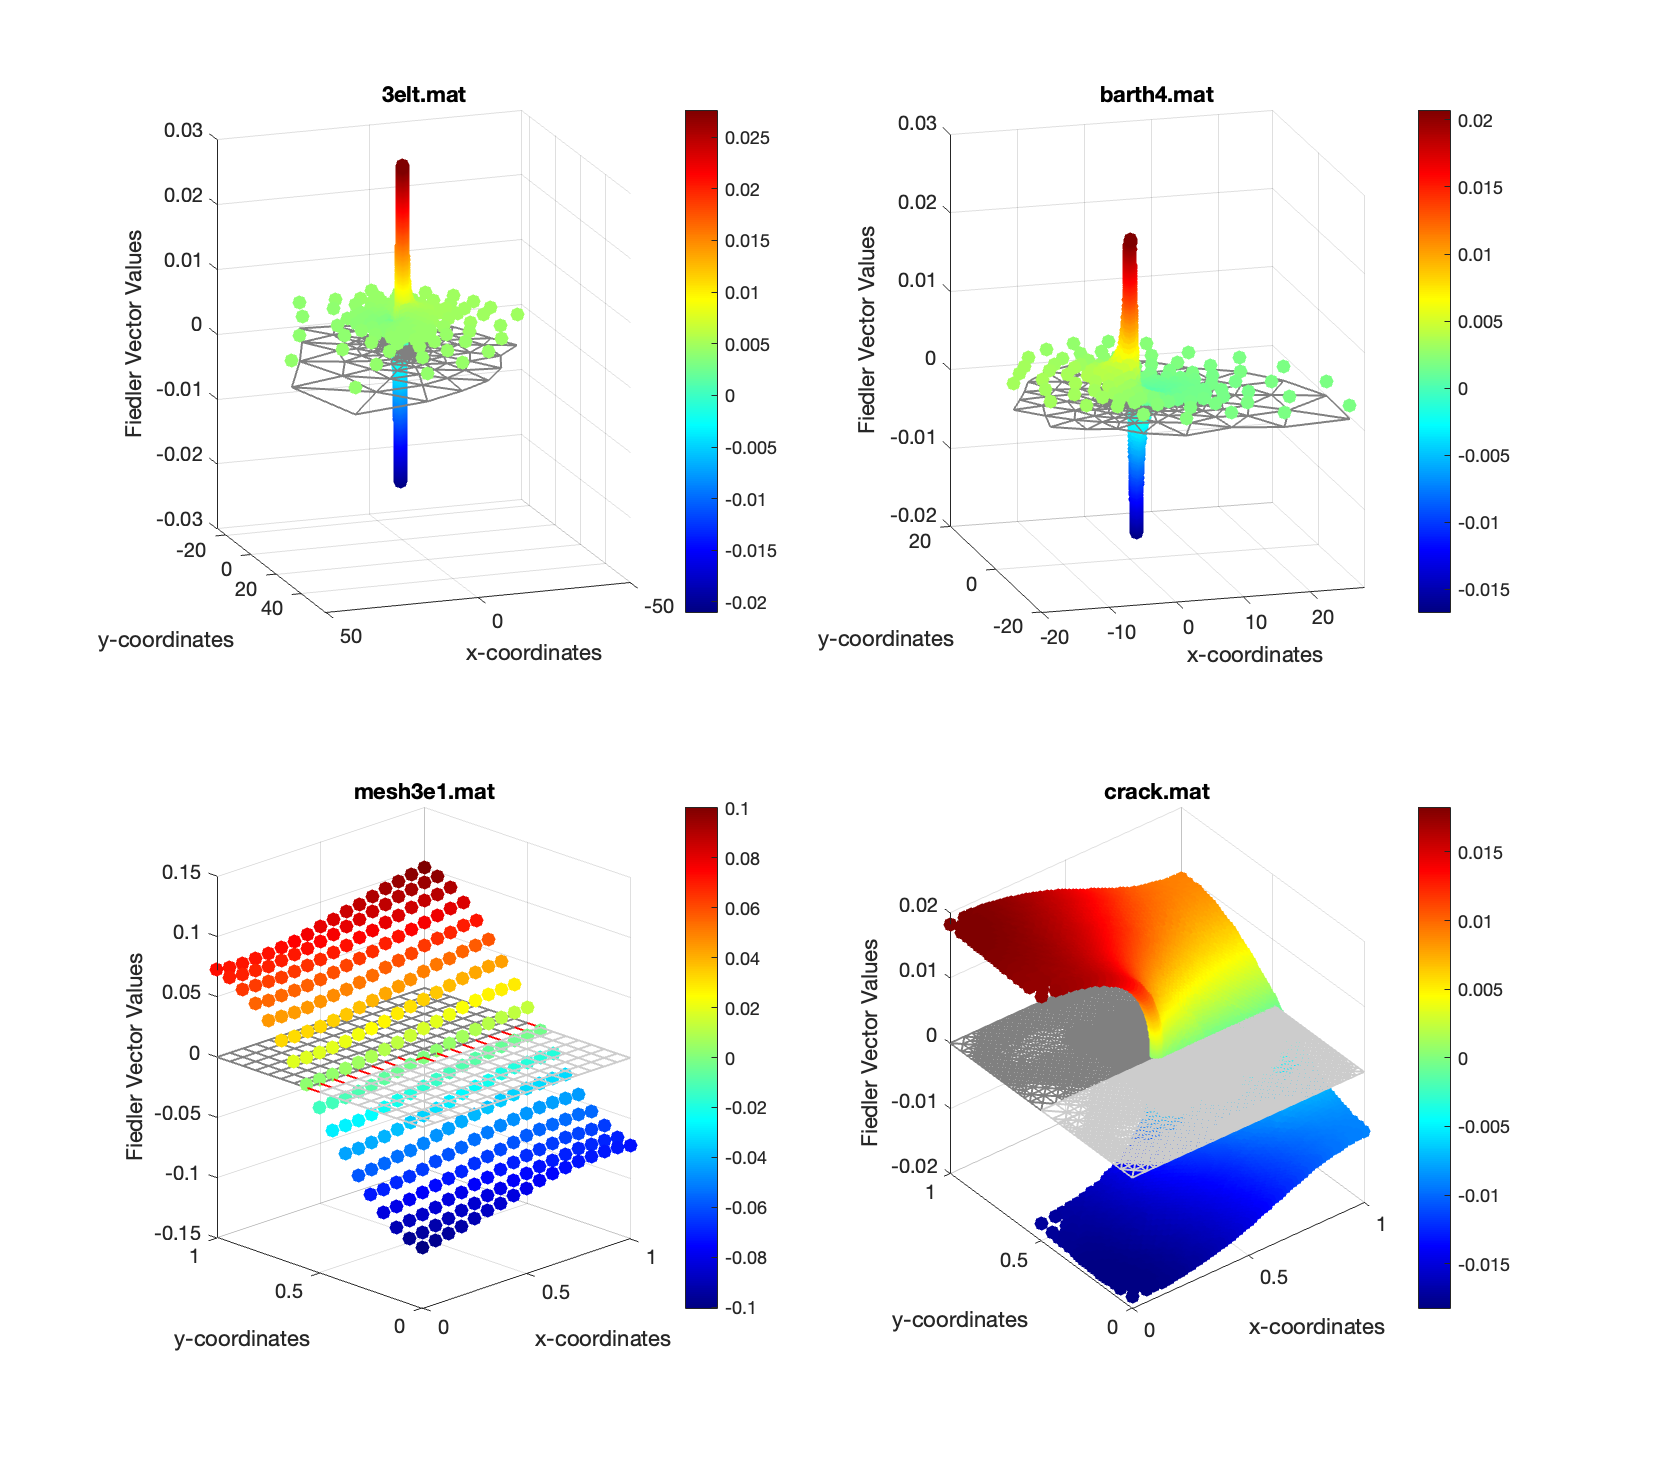
\includegraphics[width=\textwidth]{./media/fiedler.png}
	\caption{Entries of the eigenvector associated with the second smallest eigenvalue $\lambda_2$ of the Graph Laplacian matrix $L$. The two partitions are depicted in dark gray and light gray, while the cut edges is red respectively. The z-axis represents the value of the entries of the eigenvector. }
	\label{fig:proj}
\end{figure}

\begin{figure}[H]
	\centering
	\begin{subfigure}{0.5\textwidth}
		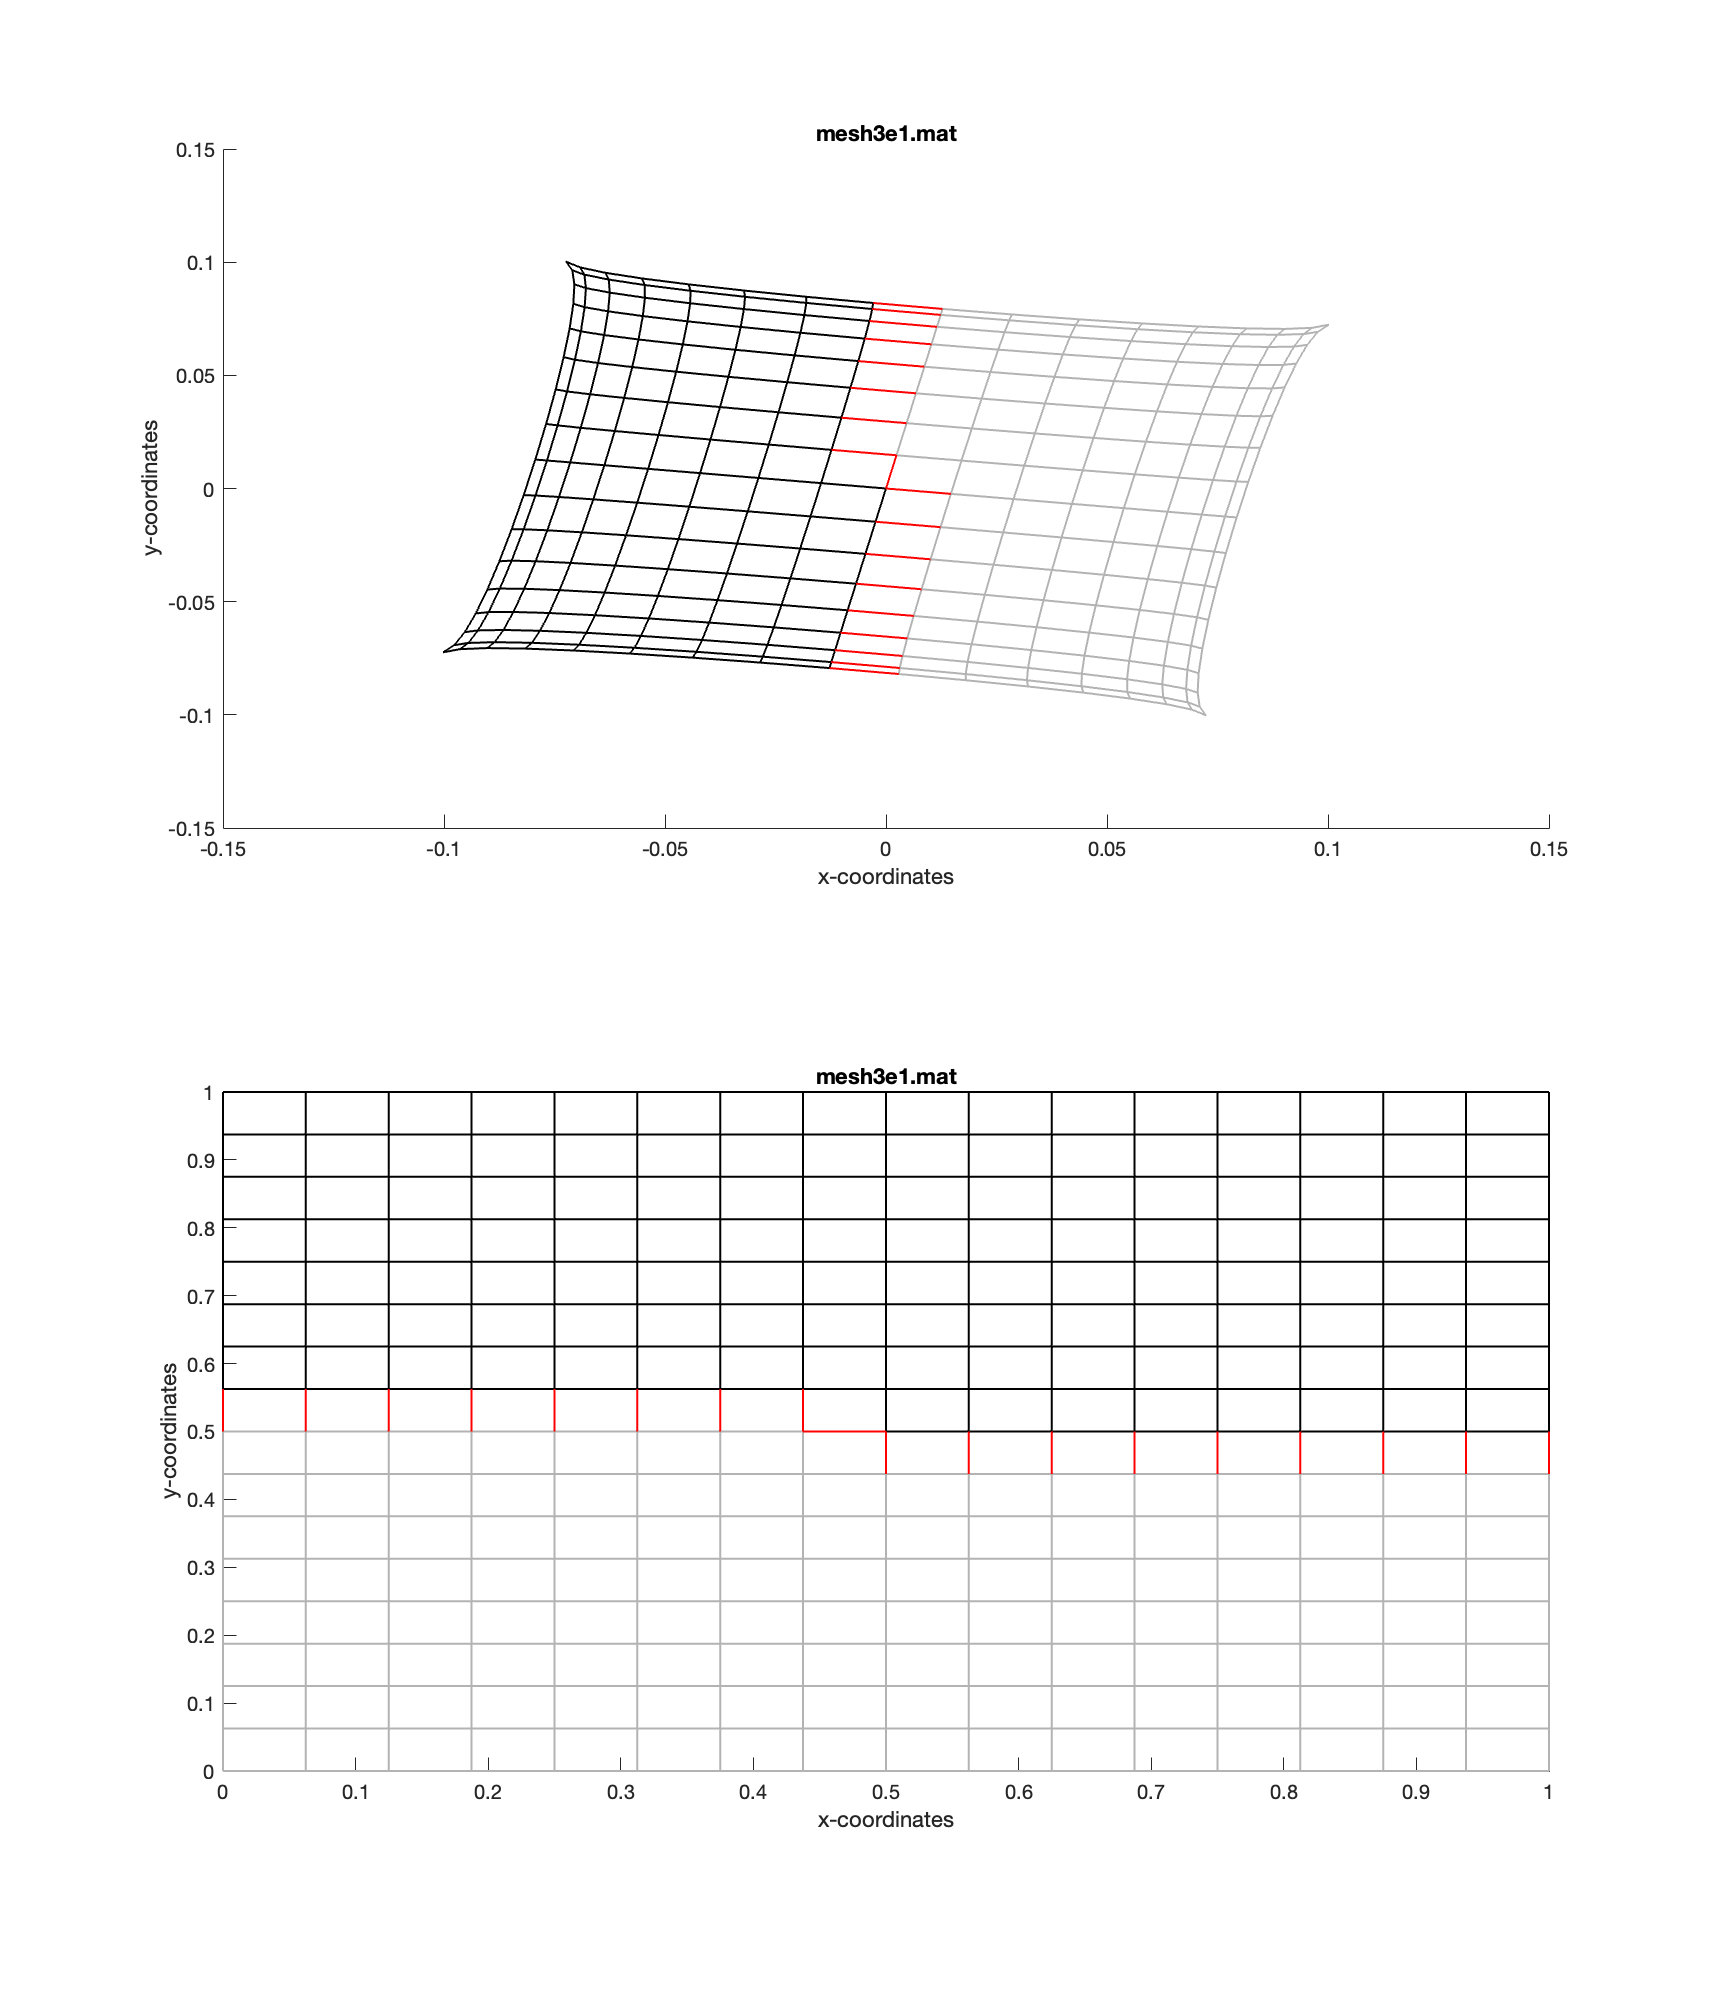
\includegraphics[width=\textwidth]{./media/mesh3e1_eigen.png}
		\caption{mesh3e1}
		\label{fig:spec_crack}
	\end{subfigure}%
	~
	\begin{subfigure}{0.5\textwidth}
		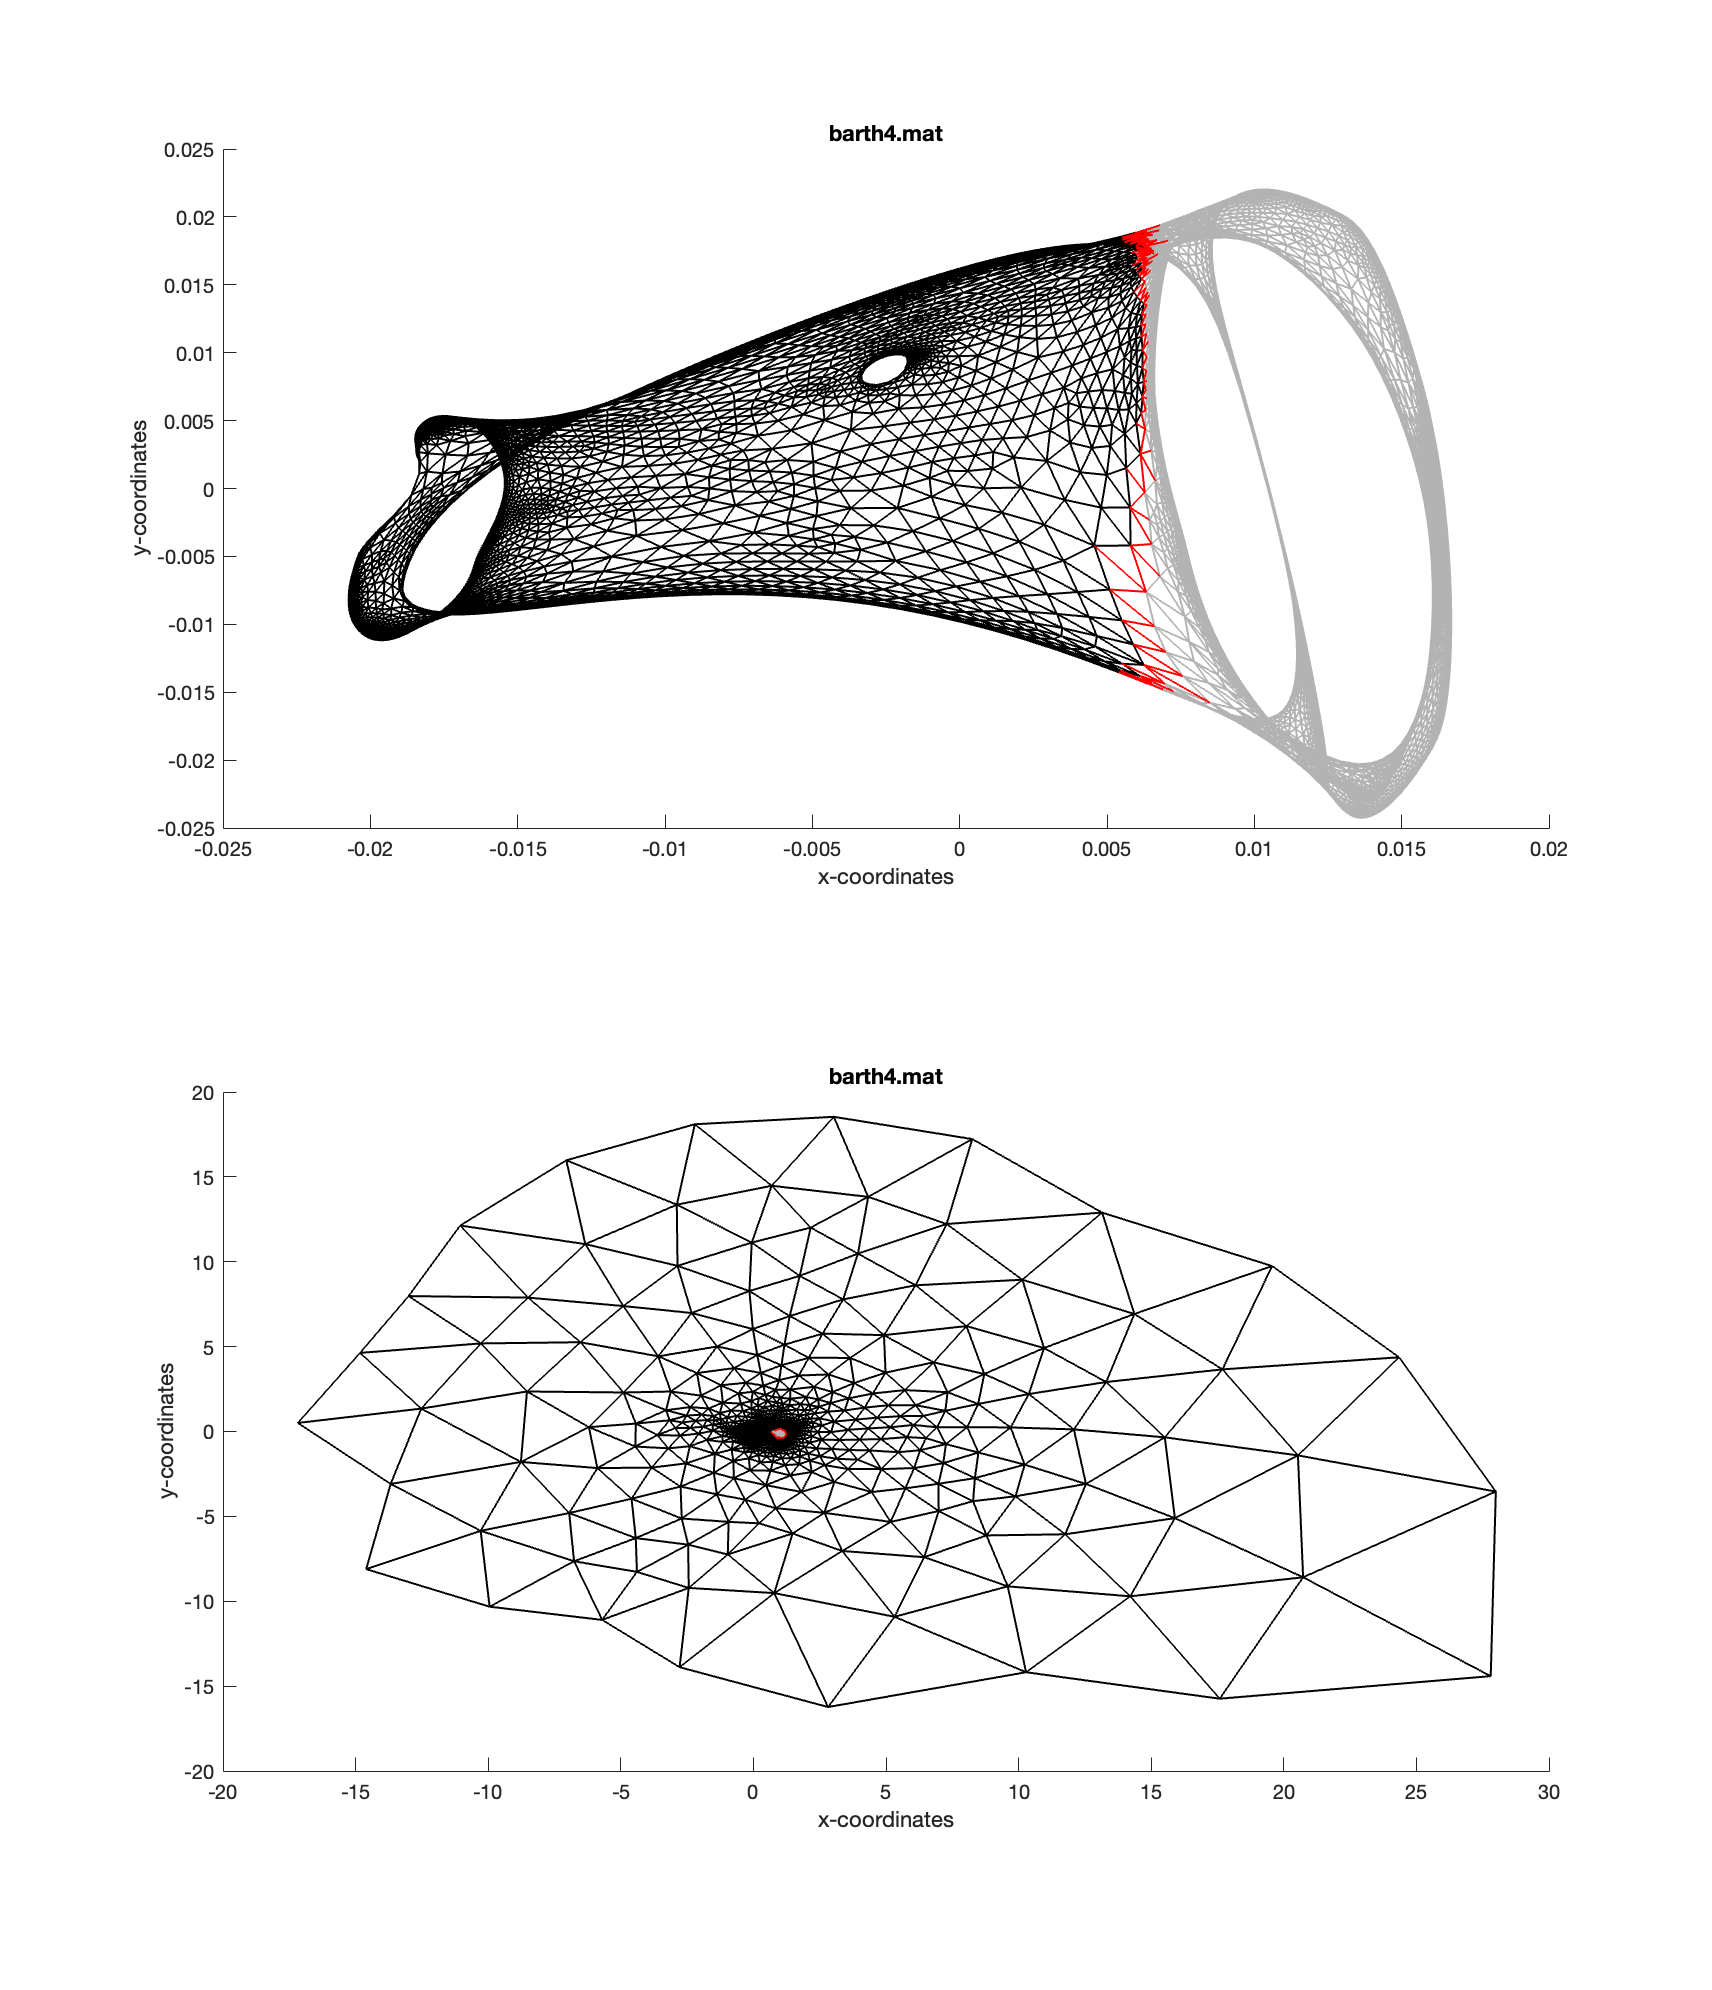
\includegraphics[width=\textwidth]{./media/barth4_eigen.png}
		\caption{barth4}
		\label{fig:barth4_spc}
	\end{subfigure}\\
	\begin{subfigure}{0.5\textwidth}
		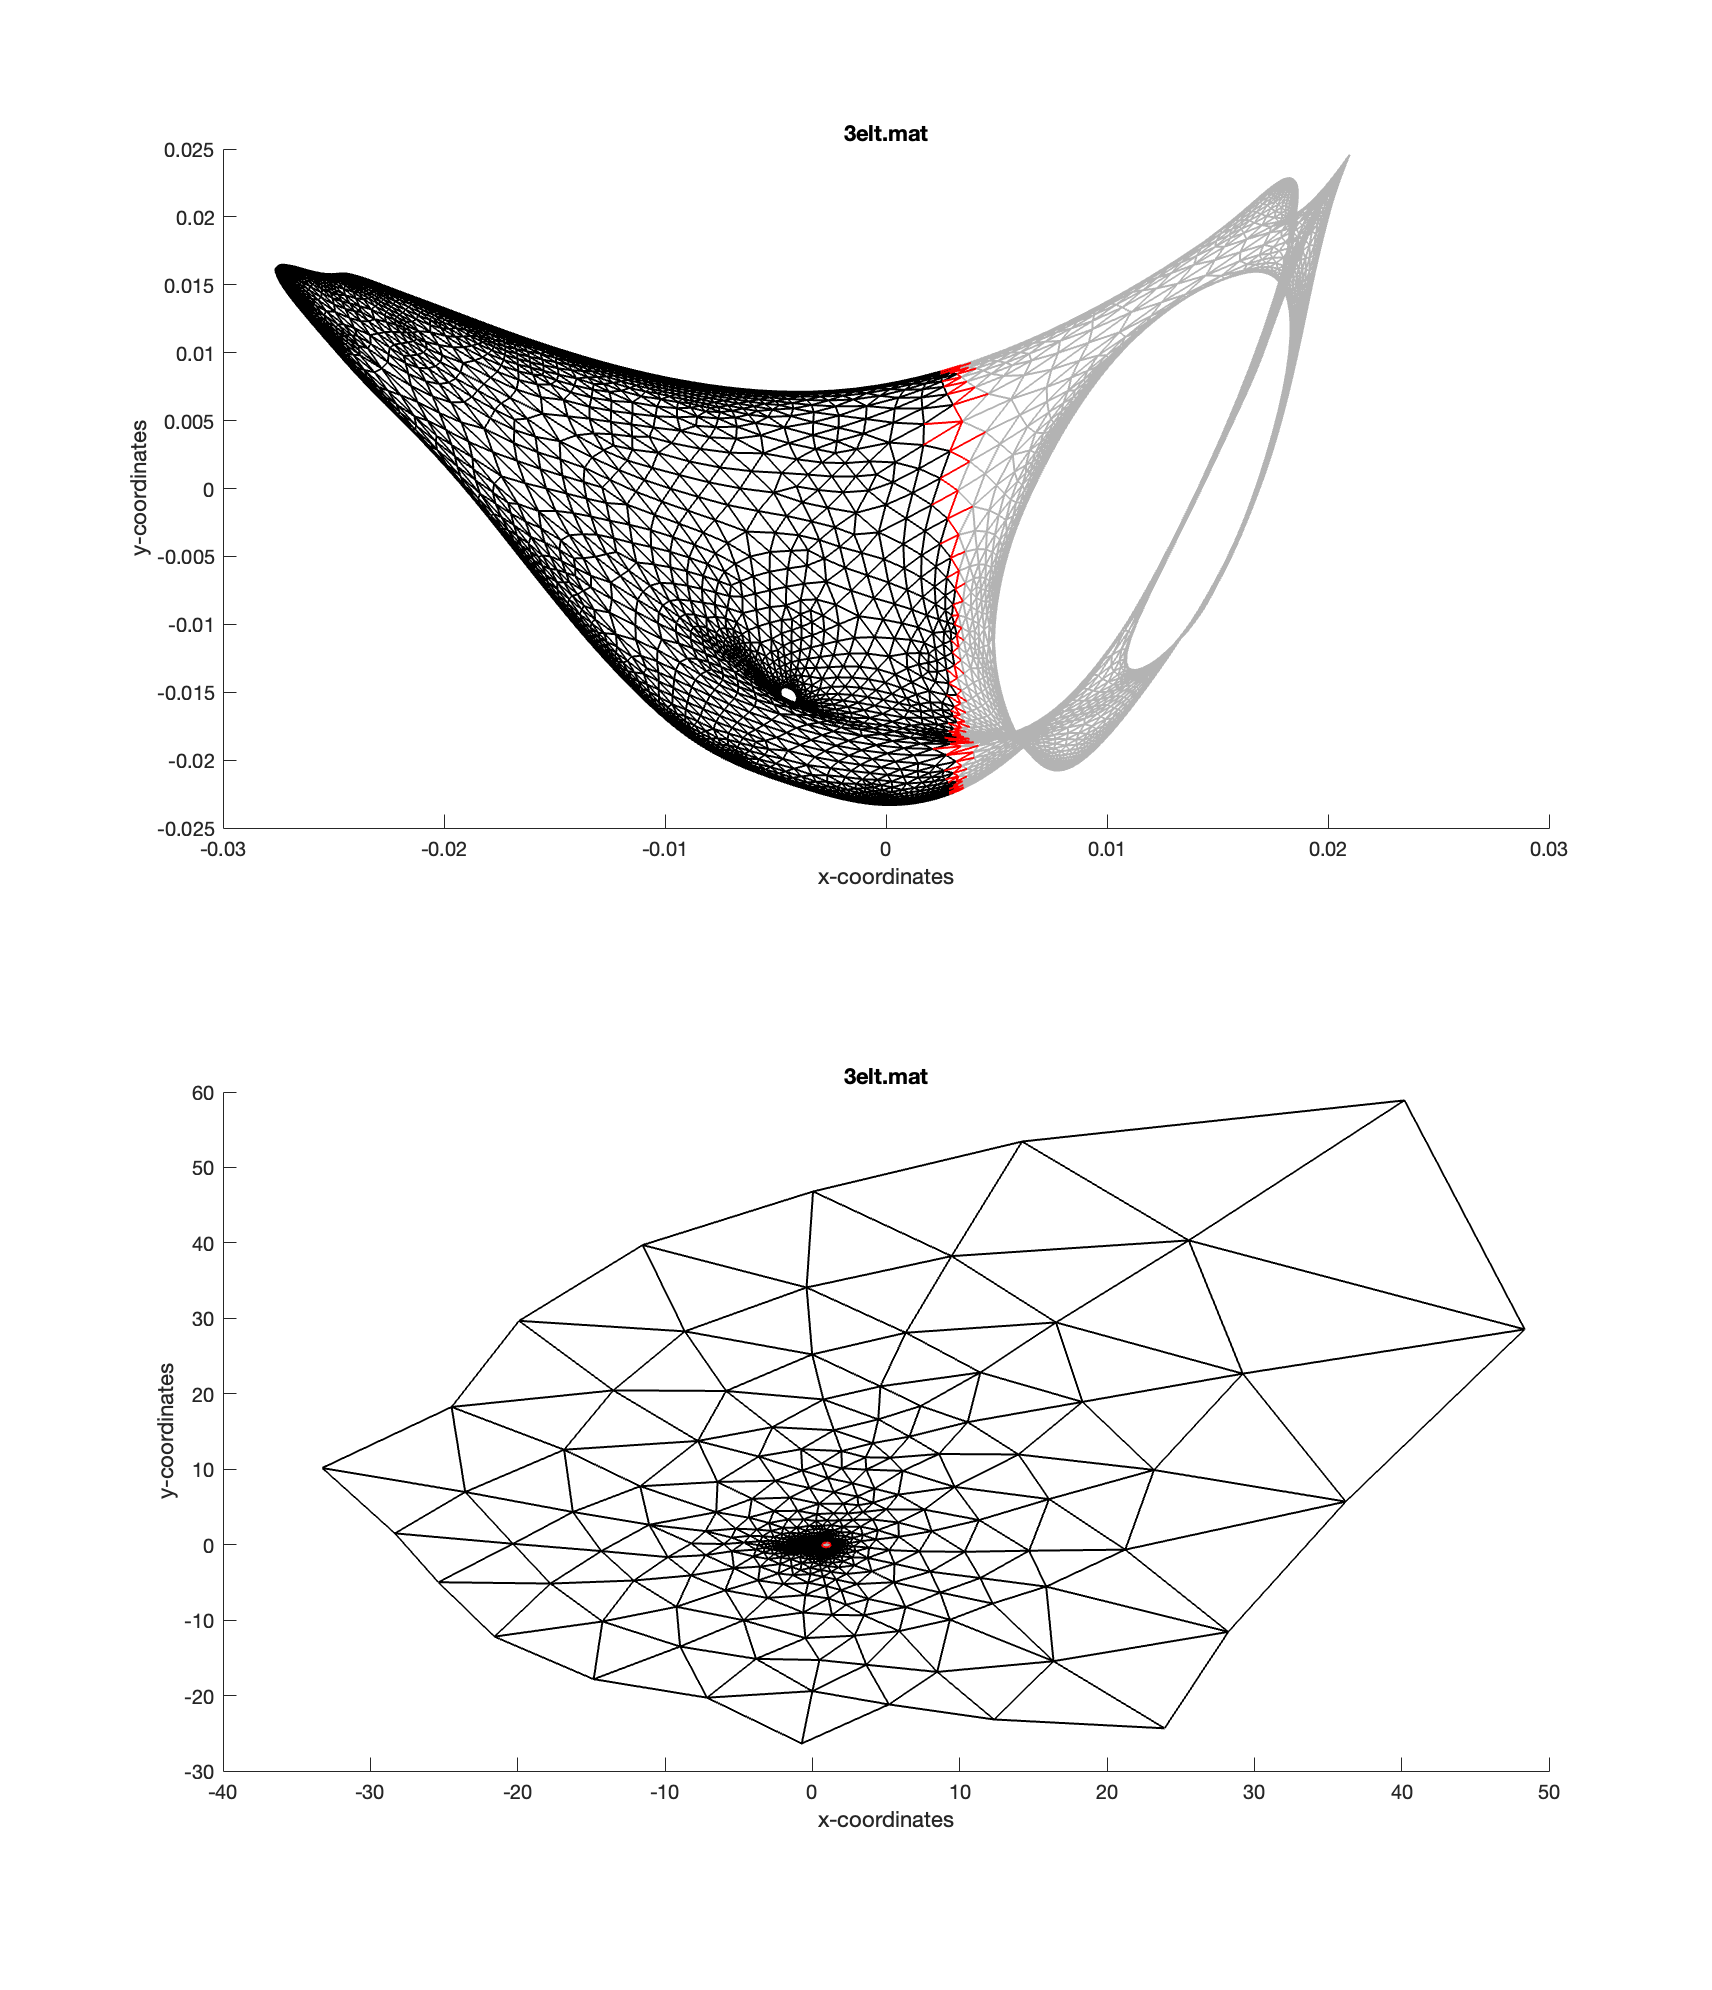
\includegraphics[width=\textwidth]{./media/3elt_eigen.png}
		\caption{3elt}
		\label{fig:metis_crack}
	\end{subfigure}%
	~
	\begin{subfigure}{0.5\textwidth}
		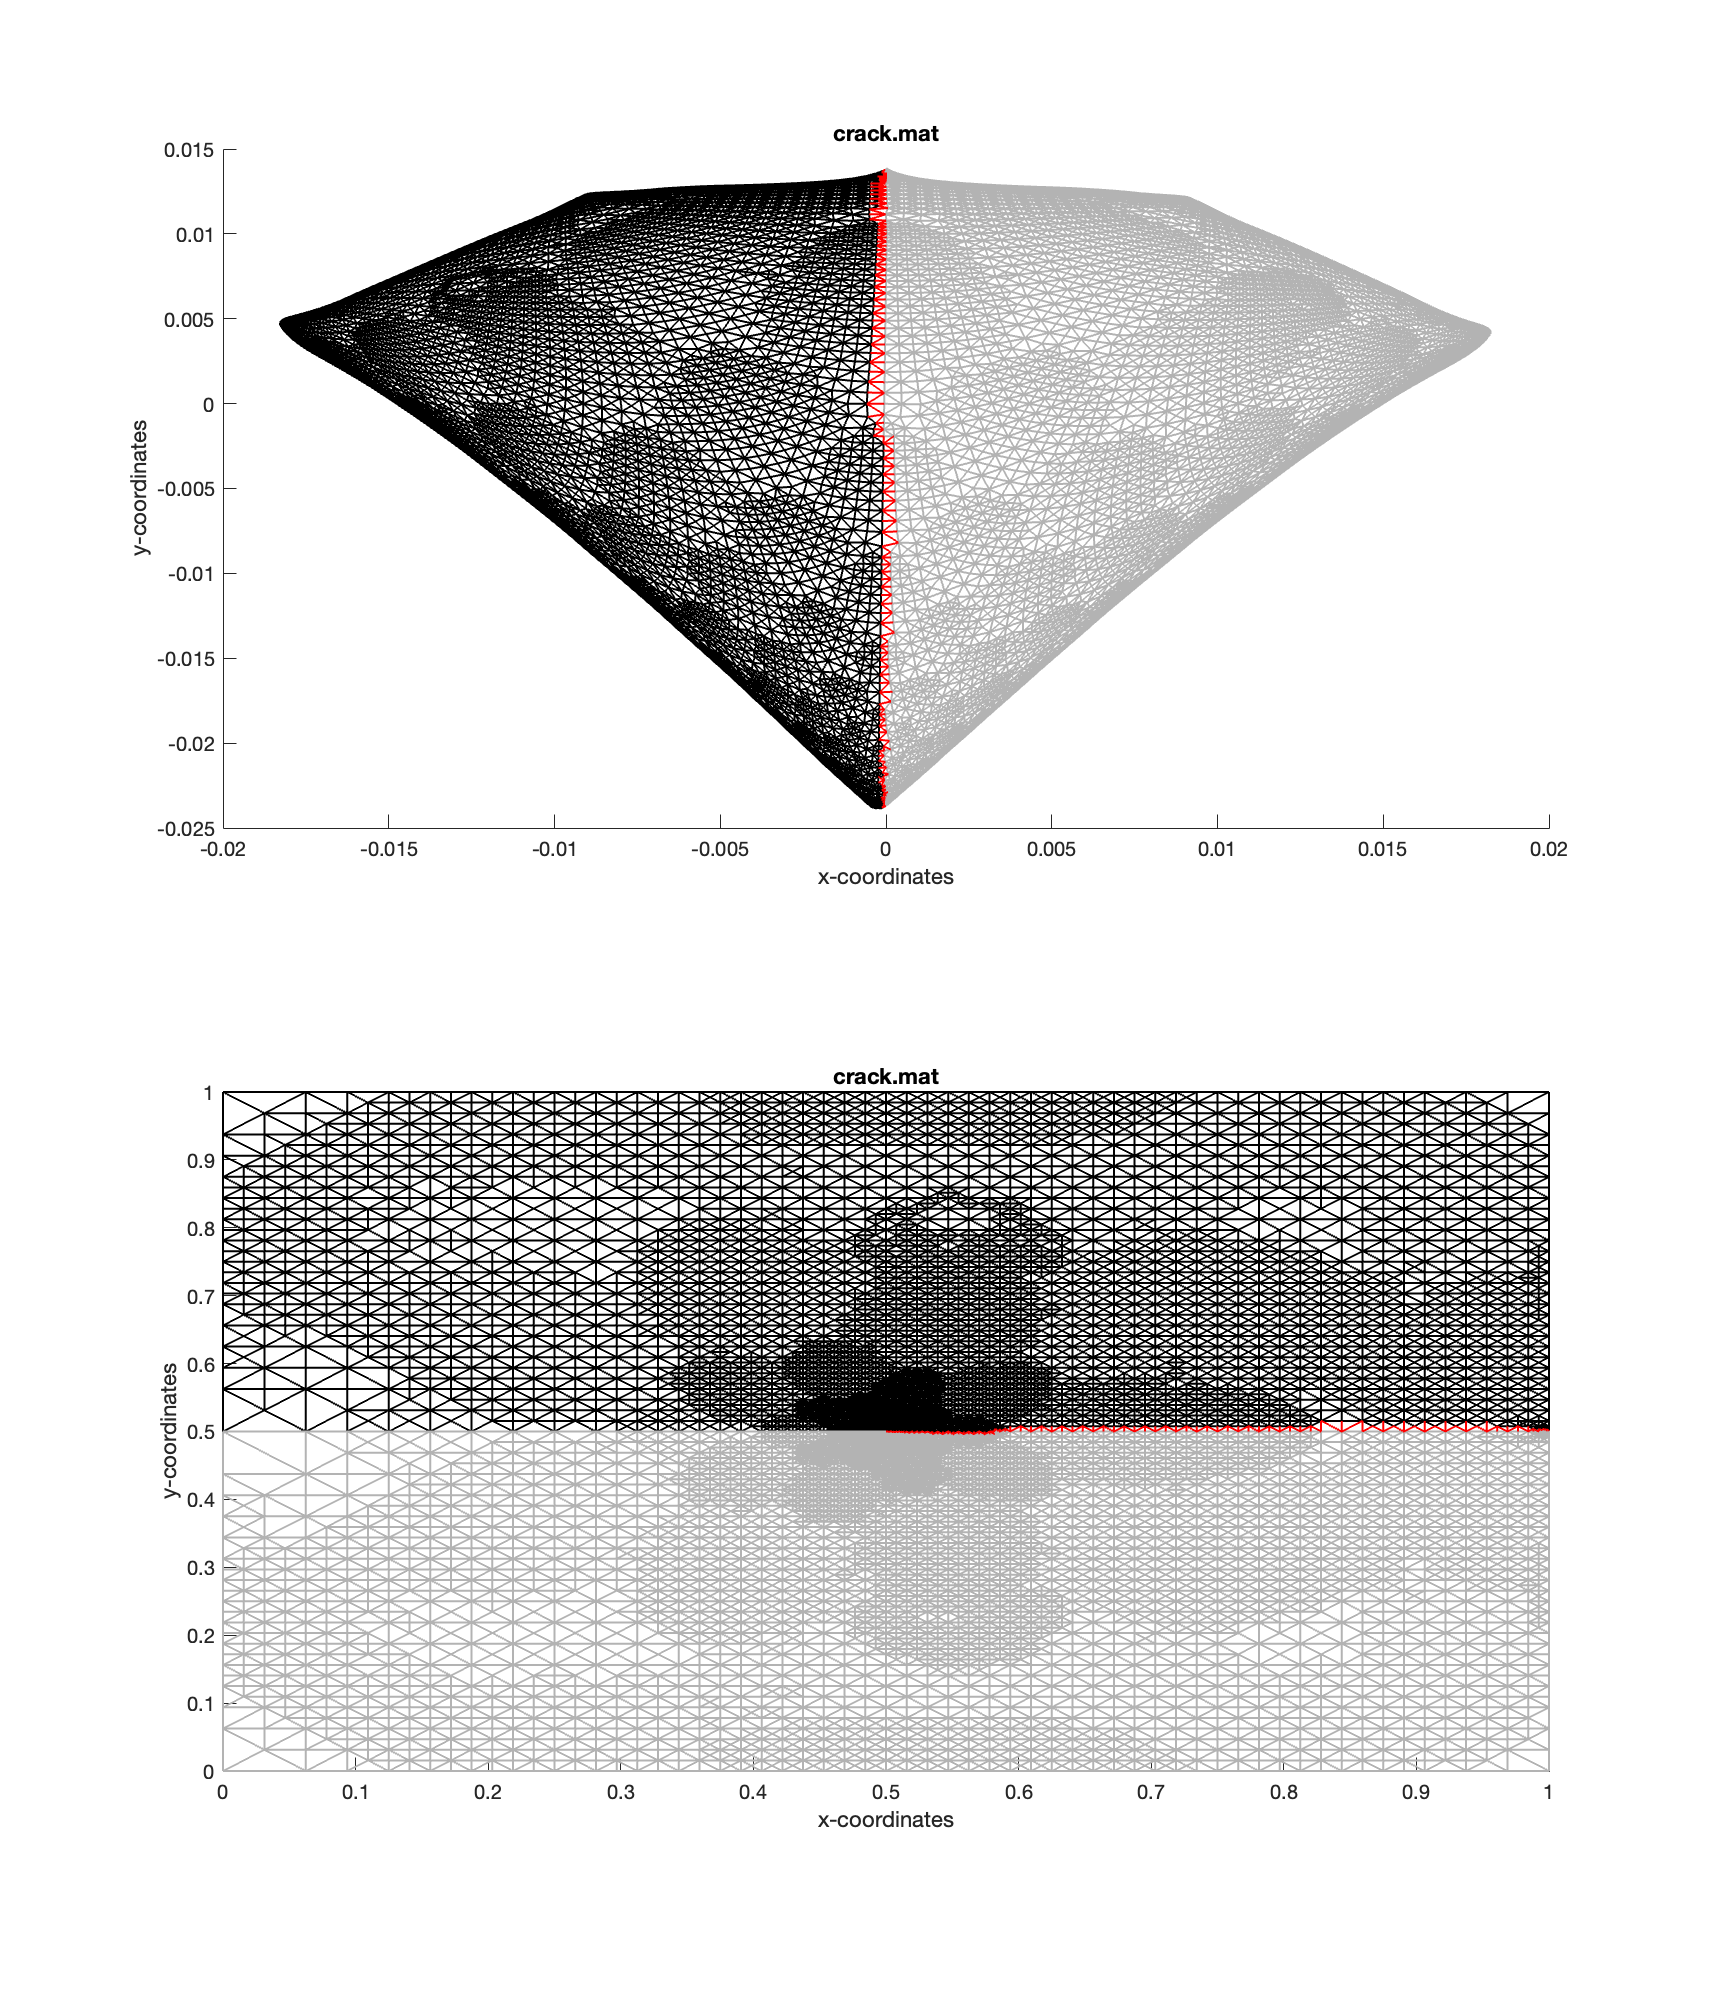
\includegraphics[width=\textwidth]{./media/crack_eigen.png}
		\caption{crack}
		\label{fig:inert_crack}
	\end{subfigure}
	\caption{Spectral bi-partitioning results using the eigenvectors to supply coordinates (top) and using cartesian coordinates (bottom).}
	\label{fig:eig_spc}
\end{figure}

